\section{Chapter Outline}
\label{sec::ChapterOutline}

Chapter \ref{ch::LiteratureReview} contains a comprehensive literature review on the background concepts. First, literature related to robotic systems is discussed in Section \ref{sec::LiteratureReview::RobotControlHRI}. Then, long-horizon task planning is discussed in the Section \ref{sec::LiteratureReview::LongHTP}. Finally, literature on Social aware navigation is discussed in the Section \ref{sec::LiteratureReview::SAN}

In Chapter \ref{ch::Contribution1}, the authors start with a literature review on behaviour-based systems in section \ref{sec::contrib1::literature}. Then, they propose a new behaviour-based planning system called "Fabric" in section \ref{sec::contrib1::methodology}. Following this, they provide the evaluation of the system in section \ref{sec::contrib1::results} and a conclusion in \ref{sec::contrib1::conclusion}.

In Chapter \ref{ch::Contribution2}, the authors start with a literature review on attention systems in section \ref{sec::contrib2::literature}. Then, they propose a new attention module called "Fabric Attention" in section \ref{sec::contrib2::methodology}. Following this, they evaluate the system in Section \ref{sec::contrib2::results} and conclude in Section \ref{sec::contrib2::conclusion}.

In Chapter \ref{ch::Contribution3}, the authors begin with a comprehensive literature review on user studies for socially aware navigation robotic systems and on user studies for the acceptance of robotic systems in section \ref{sec::contrib3::literature}. Then, they provide details on the interaction-based socially assistive robot they developed for the study, as well as the user studies they designed for system evaluation, in Section \ref{sec::contrib3::methodology}. Following this, they present the evaluation results of the survey in Section \ref{sec::contrib3::results} and provide a conclusion in Section \ref{sec::contrib3::conclusion}.

Chapter \ref{ch::ResultsAndDiscussion} contains a compilation and a summary of all the discussions detailed in previous sections.

Chapter \ref{ch::Conclusions} contains a summary of the research, achieved contribution to the research field and possible future work, 


\section{Timeline}
\label{sec::Timeline}

\begin{figure}[h]
\centering
\vspace{5mm}
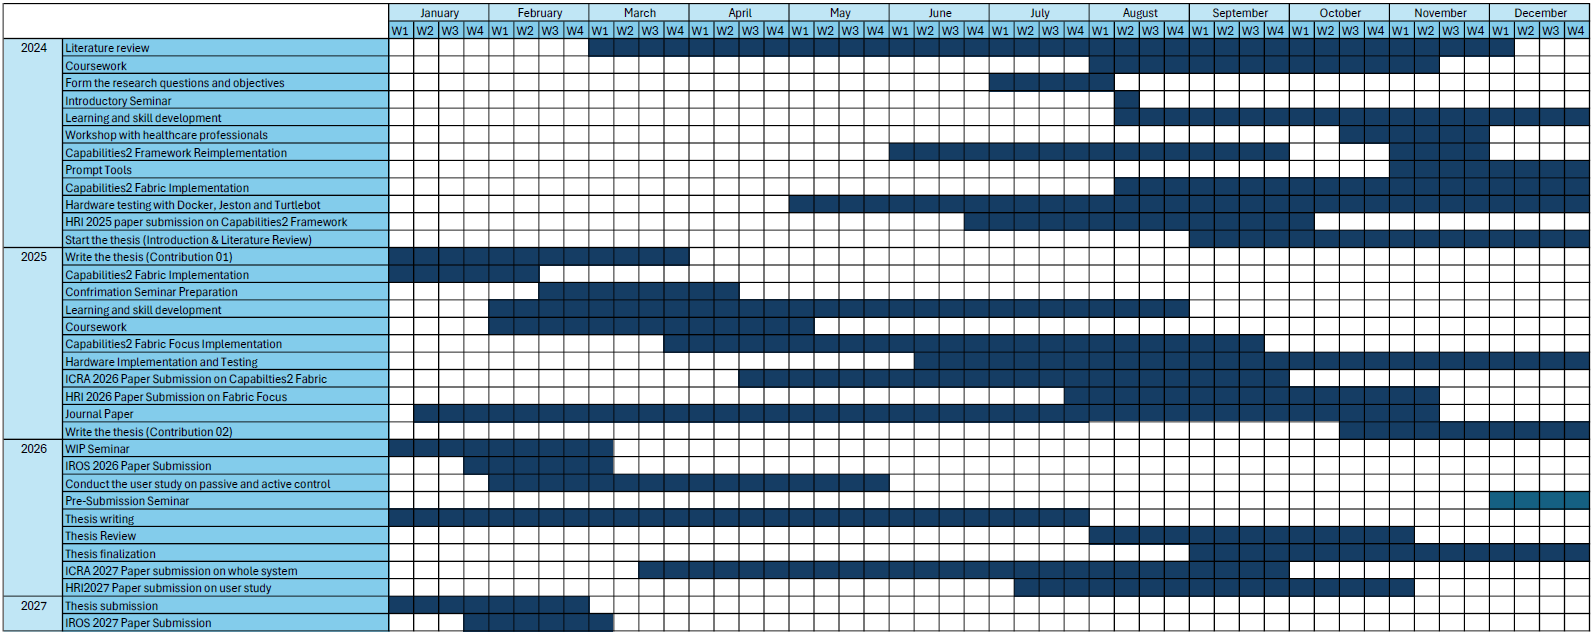
\includegraphics[width=\textwidth]{introduction/figures/timeline.png}
\caption{Expected Timeline}
\label{fig::expected_timeline}
\end{figure}